\documentclass[10pt,dvips]{beamer}
\xdefinecolor{structure}{rgb}{0.9,0.3,0.3}
\xdefinecolor{side}{rgb}{0.2,0.3,0.7}
\xdefinecolor{fond}{rgb}{0.85,0.85,0.98}

\usepackage[T1]{fontenc}
\usepackage{pst-all}
\usepackage{epsfig}
\usepackage[francais]{babel}
%\usepackage{multicol}
%\usepackage{colortab}
\usepackage{alltt}
\usepackage{amsfonts}
\usepackage{amsmath}
\usepackage{listings}
\usepackage{psfrag}
\usepackage{url}
%\usepackage[vlined]{algorithm2e}
\usepackage{array}


%\usepackage{subfigure}
%\usepackage{multirow}
\usepackage{multimedia}
%\input{macros.tex}

\newrgbcolor{brick}{0.6 0 0}
\newrgbcolor{lgray}{0.9 0.9 0.9}
\newrgbcolor{dgray}{0.45 0.45 0.45}
\newrgbcolor{links}{0. 0. 0.60}
\newlength{\myHeight}

\newcommand{\dcite}[1]{{\color{blue}{\cite{#1}}}}



\setbeamertemplate{navigation symbols}{}

\beamertemplatetransparentcovereddynamic



\definecolor{lg}{RGB}{220,220,220}
\definecolor{lred}{RGB}{250,150,150}
\definecolor{lblue}{RGB}{150,150,250}
\definecolor{dblue}{RGB}{30,30,100}
\definecolor{dgreen}{RGB}{30,100,30}



\newcommand{\citeb}[1]{\mbox{\em \color{blue}{\cite{#1}}}}
\newcommand{\Cite}[1]{\mbox{\em \color{blue}{ #1 }}}
\newcommand{\Etal}[0]{\mbox{\em et. al.}}

\newcommand{\AlertB}[1]{{\color{blue} #1}}
\newcommand{\AlertM}[1]{{\color{mmagenta} #1}}
\newcommand{\AlertR}[1]{{\color{brick} #1}}



\newcommand{\class}[1]{{\color{brick}{\texttt{#1}}}}





\setbeamercovered{transparent}


\newcommand{\surligne}[2]{%
\colorbox{#1}{#2}}


\newcommand{\ligne}[1]{
  \rput#1{\psline[linewidth=0.05,linecolor=black,fillstyle=solid](0.0,0.0)(0.3,0.0)}}
\newcommand{\point}[1]{
  \rput#1{\psline[linewidth=0.1,linecolor=black,fillstyle=solid](0.0,0.0)(0.1,0.0)}}



\beamertemplateshadingbackground{gray!1}{structure!5}
\usetheme{CambridgeUS}





\begin{document}



\mode<presentation>

\title[Flux, visualisation 3D]{Flux, visualisation 3D }
\author[B. Kerautret ]{Bertrand Kerautret\inst{1,2} }
\date[2$^{iem}$Journ�es DGtal-2011 ]{{\small{Journ�es DGtal, 29 aout-2 septembre 2011 }}}
\institute[LORIA-LAMA]{\inst{1} LORIA - Nancy University \\ 
  \inst{2} LAMA - University of Savoie }


\frame{
\titlepage
\rput(6,0){
\includegraphics[width=3.5cm]{Images/dgtal.eps}} 

}





\section{1. Visualisation 3D: contexte, orientation}


\subsection{Contexte}


\begin{frame}[t]
\frametitle{1. Visualisation 3D: contexte}
\vspace{-0.3cm}
\begin{block}{Premier \textit{DGtal meeting} (4 janvier 2011)}
\begin{itemize}
\item Outils de visualisation pour les primitives 2D.
\item M�canisme simple permettant de montrer des r�sultats li�s � diff�rents modules:  
\begin{itemize}
\item Topologie (Jacques-Olivier lachaud)
\item G�om�trie (David Coeurjolly, Tristan Roussillon)
\item Domaine (Guillaume Damian)
\end{itemize}
\end{itemize}
\end{block}

\visible<2>{\rput(6,-1.7){
\begin{minipage}{\textwidth}
\begin{center}
\begin{tabular}{ccc}
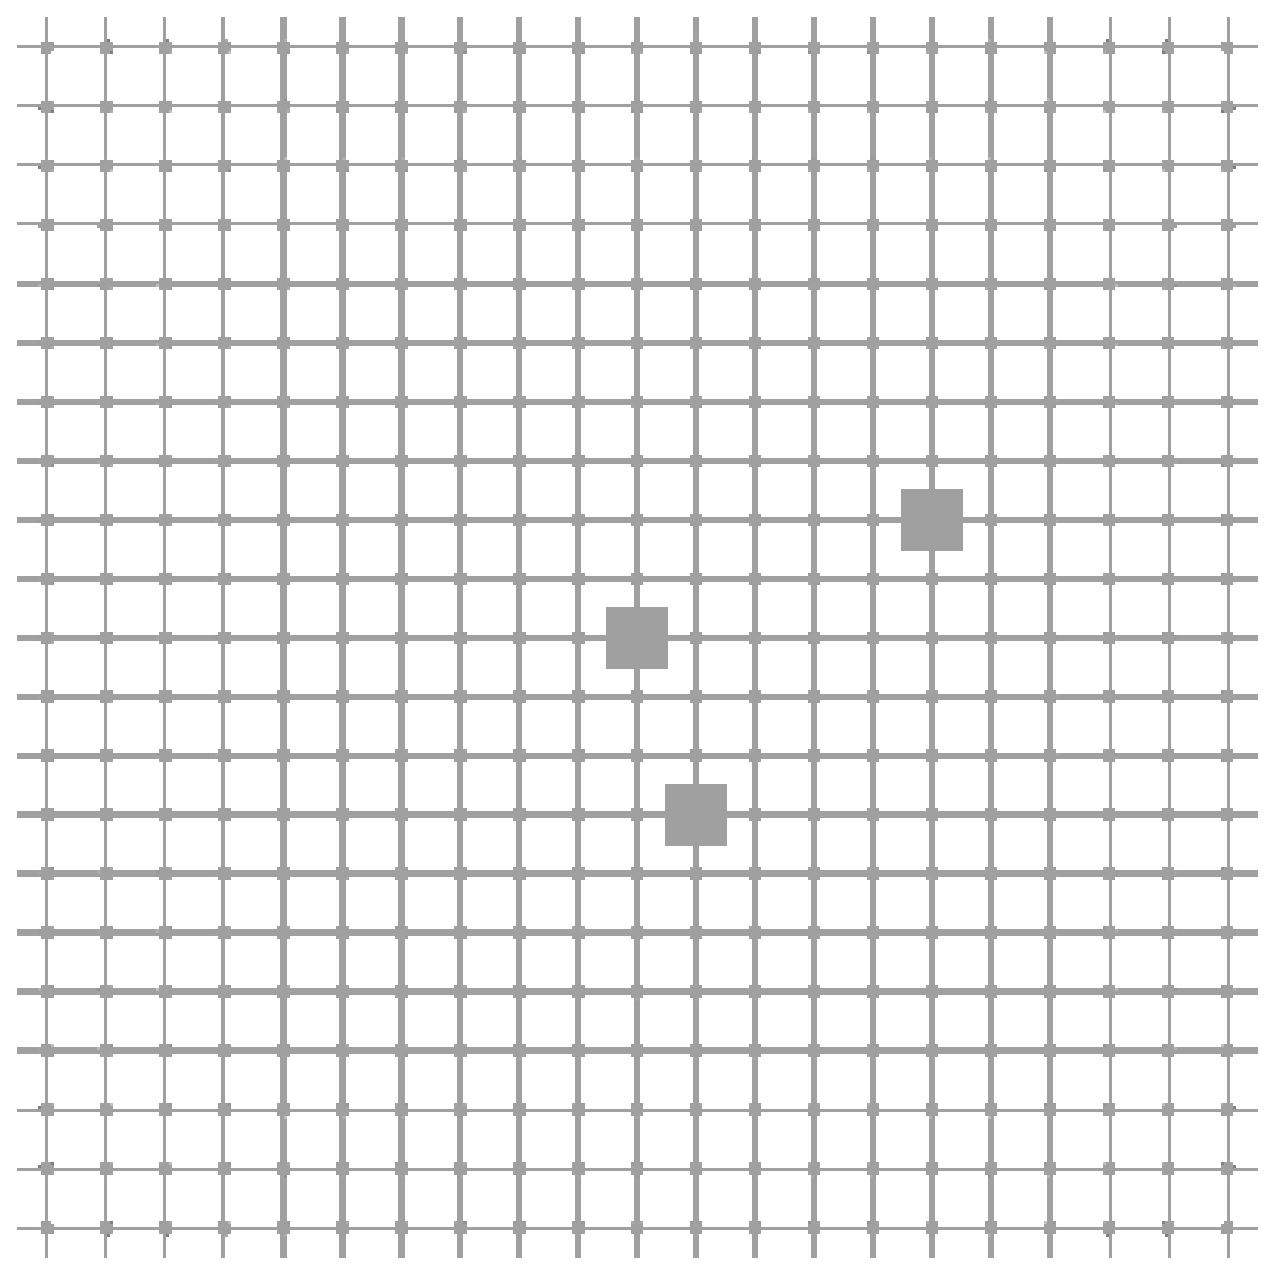
\includegraphics[height=0.15\textwidth]{Images/gallerie1.eps}&
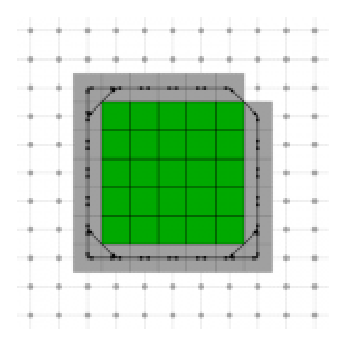
\includegraphics[height=0.15\textwidth]{Images/gallerie2.eps}&

\includegraphics[height=0.15\textwidth]{Images/gallerie3.eps}\\
$\vcenter{ \hbox{
\includegraphics[height=0.15\textwidth]{Images/gallerie4.eps}}}$ &
$\vcenter{ \hbox{\includegraphics[height=0.1\textwidth]{Images/gallerie5.eps}}}$ &
$\vcenter{ \hbox{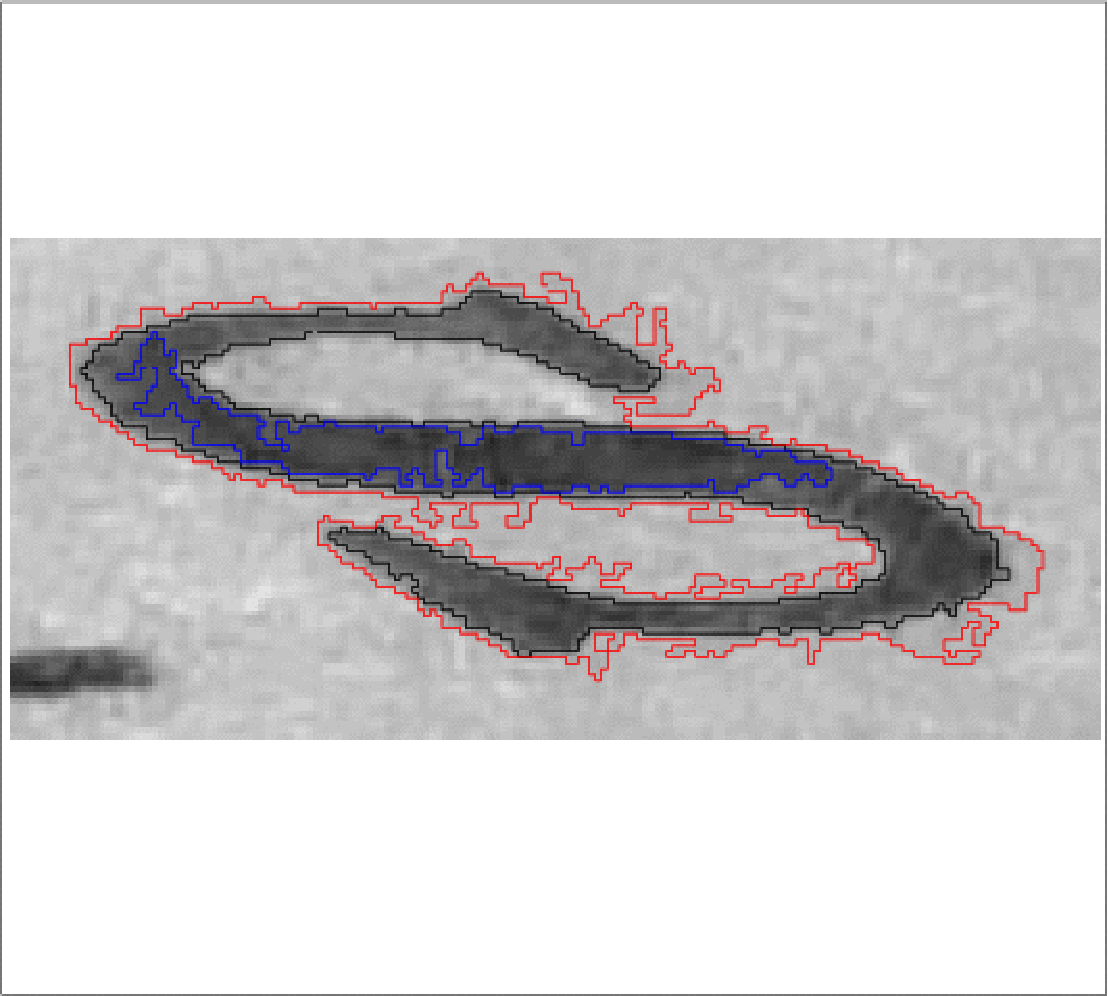
\includegraphics[height=0.15\textwidth]{Images/gallerie6.eps}}}$ \\
\end{tabular}
\end{center}
\end{minipage}}}
\vspace{-0.3cm}

\visible<3->{
\begin{block}{Objectifs pour la visualisation  3D}
\begin{itemize}
\item Garder un syst�me simple par flux (m�me primitive).
\item Manipulation, �dition d'objet 3D. 
\item Plusieurs directions: 
\begin{itemize}
\item Bertrand Kerautret: visualisation bas�e \textit{OpenGL, LibQGLviewer}
\item Jacques-Olivier Lachaud: visualisation bas�e \textit{Open Inventor SoQT}
\item Martial Tola: visualisation (2D/3D) bas�e sur \textit{CAIRO \footnote{Biblioth�que de rendu vectoriel: \url{http://cairographics.org}}}  


\end{itemize}
\end{itemize}

\end{block}
}
\end{frame}









\subsection{Orientation}


\begin{frame}[t]

\frametitle{1. Visualisation 3D: objectif}

{\large{Inspir� du m�canisme de \texttt{Board2D} (initialement bas� sur \texttt{LibBoard}\footnote{(Copyleft, LGPL) 2007 S�bastien Fourey - GREYC ENSICAEN}) }}

\begin{block}{}
\begin{itemize}
\item Chaque primitive capable de s'auto dessiner. 
\item V�rifier le concept \texttt{CDrawableWithBoard2D} (concept v�rifi� avec \textit{\textcolor<3>{red}{boost}}).  
\item<4-> M�canisme de ``flux'' avec l'op�rateur \texttt{< \hspace{-0.2cm}<}.
\item<6-> Exportation en diff�rents formats (pdf, eps, fig, gif, png). 
\end{itemize}
\end{block}


\visible<2,3>{%
\begin{footnotesize}
\begin{itemize}
\item \texttt{std::string styleName() const}
\item \texttt{DrawableWithBoard2D* defaultStyle(const std::string \& mode = "" ) const}
\item \texttt{void selfDraw( Board2D \& ) const}
\item<3> \texttt{\color{red}{BOOST\_CONCEPT\_ASSERT((CDrawableWithBoard2D<TDrawableWithBoard2D>));}}
\end{itemize}
\end{footnotesize}

}

\visible<5->{%
\visible<6,7>{\rput(3;6){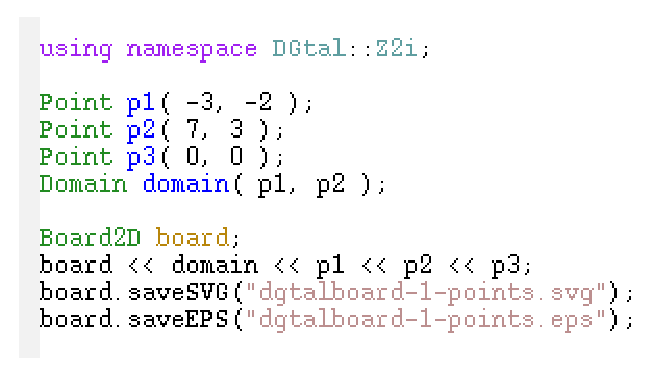
\includegraphics[width=6cm]{Images/codeExBoard2D.eps}}}%
\visible<7>{\rput(9;4){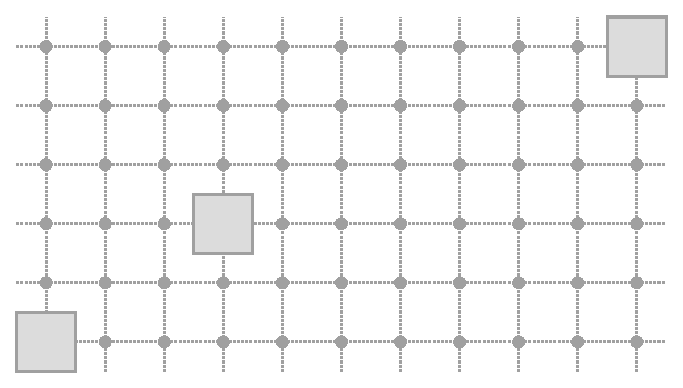
\includegraphics[width=5cm]{Images/dgtalboard-1-points.eps}}}%
\visible<5>{\rput(3;9){
\begin{minipage}{0.5\textwidth}
\begin{itemize}
\item[] \texttt{\footnotesize{Board2D board;}} 
\item[] \texttt{\footnotesize{board \texttt{< \hspace{-0.2cm}<} object;}} 
\end{itemize}%
\end{minipage}}}
}%

\end{frame}






\section{2. Principe de la visualisation 3D}



\begin{frame}[t]
\frametitle{2. Principe de la visualisation 3D}
\begin{block}{M�canisme comparable en 3D:}
\begin{itemize}
\item Classe semie abstraite: \class{Display3D}
\item M�me principe: op�rateur \texttt{< \hspace{-0.2cm}<} et concept \class{CDrawableWithDisplay3D}
\item Deux classes h�ritent de \class{Display3D}: \class{Viewer3D} et \class{Board3D2D}  
\end{itemize}
\end{block}
\only<1,2,3>{\visible<2-> { \begin{block}{Visualisation bas�e \textit{OpenGL}: \class{Viewer3D}}
\begin{itemize}
\item Utilisation de la biblioth�que \textit{LibQLViewer} \footnote{\url{http://www.libqglviewer.com}}
\item H�rite � la fois de \texttt{Display3D} et \texttt{QGLViewer}.
\item<3> [+] Visualisation 3D interactive (possibilit� de s�lectionner des objets 3D). 
\item<3> [+] Fonctionnement simple.
\item<3> [+] Toujours maintenue depuis 2005 (derni�re version Juin 2010). 
\item<3> [-] D�pendance avec \textit{QT}. 
\item<3> [-] Export vectoriel possible (th�oriquement mais limit�).
\end{itemize}\end{block}}}%
\only<4>{
\begin{block}{Visualisation bas�e \textit{CAIRO}:  \class{Board3DTo2D} (Martial Tola)}
\begin{itemize}
\item M�me principe mais pas d'interaction.
\item [+] Pas de d�pendance \textit{QT}/carte 3D. 
\item [+] Export qualit� vectoriel.
\item [-] Positionnement manuel de la cam�ra. 
\item [-] Potentiellement moins riche compar� � \textit{OpenGL}. 
\end{itemize}
\end{block}
}
\end{frame}



\begin{frame}
\frametitle{2. Principe de la visualisation 3D}

\begin{block}{Classes v�rifiant le concept \class{CDrawableWithDisplay3D} }
\begin{center}
\begin{tabular}{lcc}
Classe & 3DViewer & Board3DTo2D \\
\class{PointVector} & X & X \\
\class{DigitalSetBySTLSet} & X & X \\
\class{DigitalSetBySTLVector} & X & X \\
\class{Object} & X & X \\
\class{HyperRectDomain} & X & X \\
\class{KhalimskyCell} & X & bient�t \\
\class{SignedKhalimskyCell} & X & bient�t
\end{tabular}
\end{center}

\end{block}


\end{frame}





\begin{frame}
\frametitle{Exemple de visualisations 3D}
\only<1>{
\begin{block}{Visualisation bas�e \class{Viewer3D}}
\begin{center}
\begin{tabular}{cc}
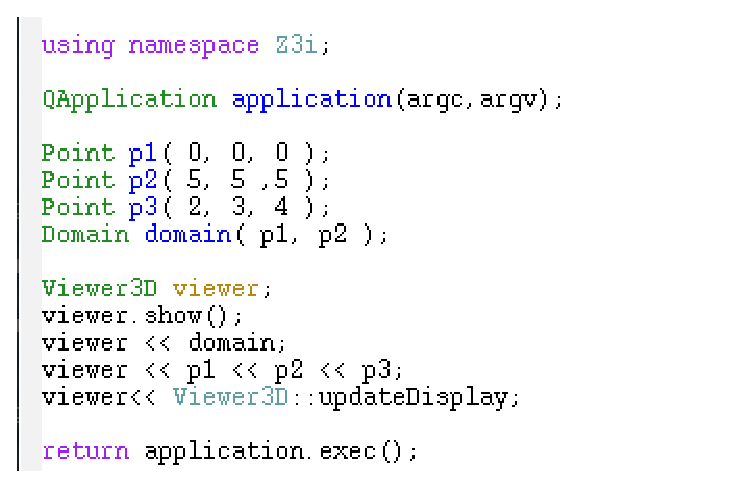
\includegraphics[height=0.33\textwidth]{Images/codeEx3DViewer.eps}&
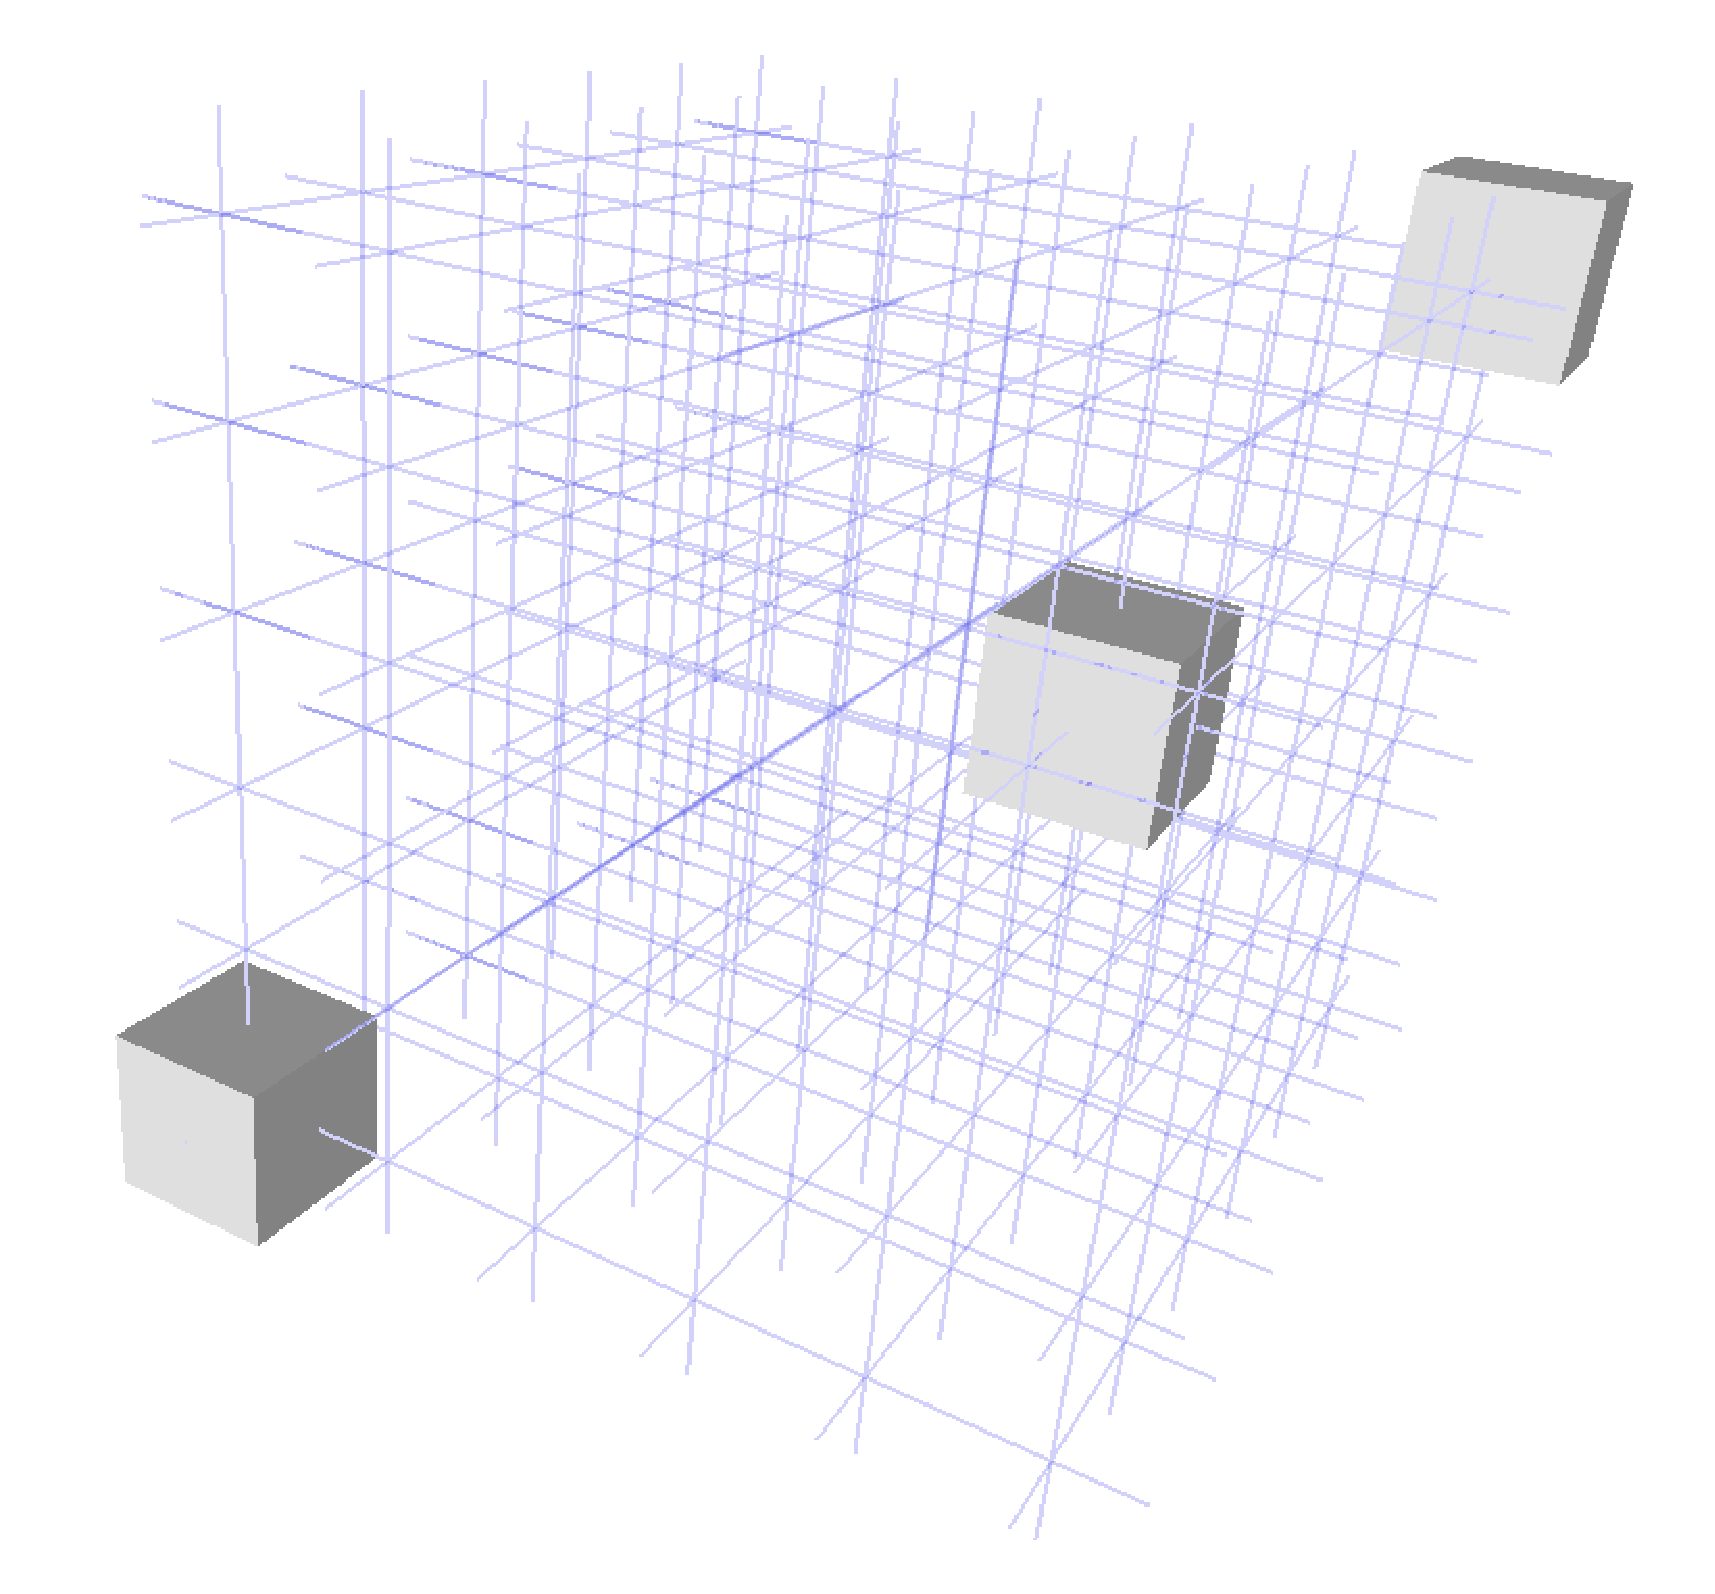
\includegraphics[height=0.33\textwidth]{Images/simple3dVisu1.eps}
\end{tabular}
\end{center}
\end{block}}

\only<2>{
\begin{block}{Visualisation bas�e \class{Board3DTo2D}}
\begin{center}
\begin{tabular}{cc}
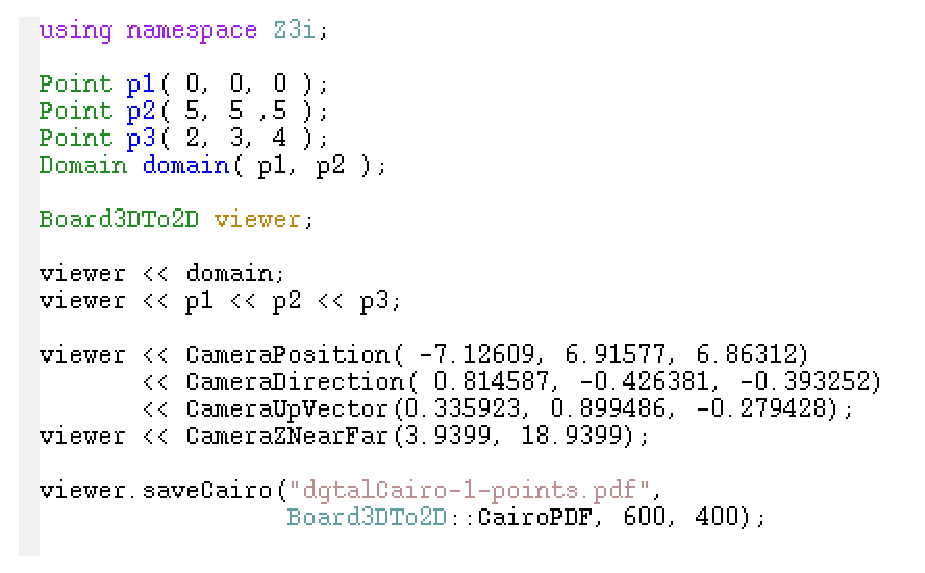
\includegraphics[height=0.33\textwidth]{Images/codeExBoard3D.eps}&
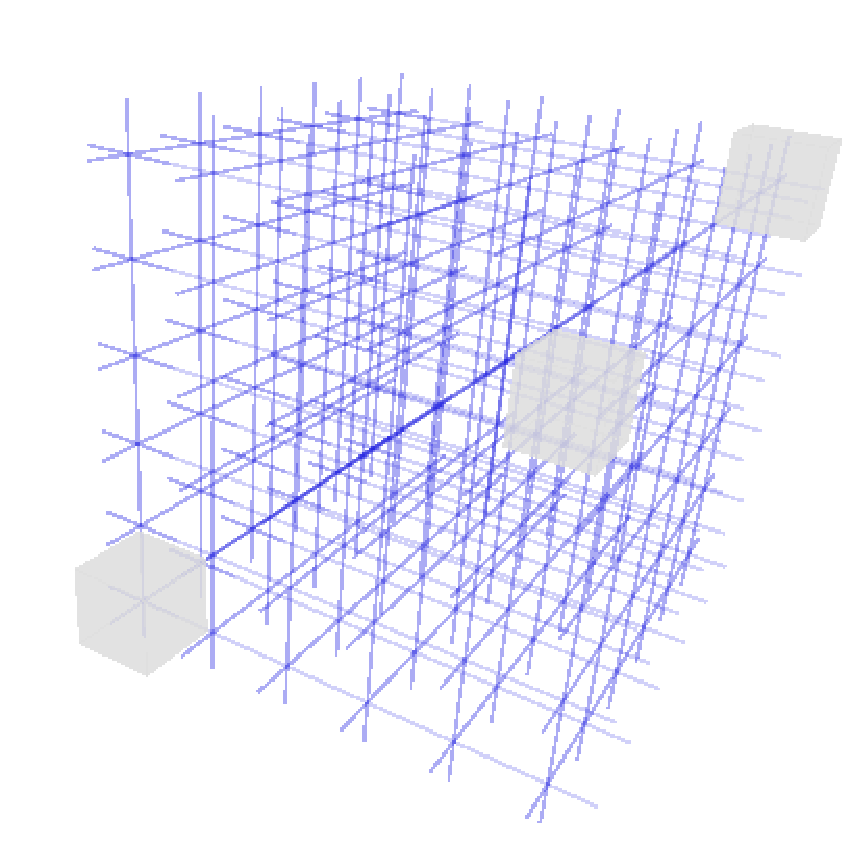
\includegraphics[height=0.33\textwidth]{Images/dgtalCairo-1-points.eps}
\end{tabular}
\end{center}
\end{block}
}

\end{frame}







\section{3. Modes de visualisation 3D}





\begin{frame}
\frametitle{3. Modes de visualisation 3D}

\begin{block}{Modification du style d'affichage}
D�finie pour chaque primitive:
\begin{semiverbatim}
viewer  \texttt{< \hspace{-0.2cm}<}  SetMode3D( p1.styleName(), "Grid" );
\end{semiverbatim}

\end{block}

\begin{block}{Diff�rents modes possibles: }
\begin{center}
\begin{tabular}{l|l}
Classe & modes \\ \hline

\class{PointVector} &  "Paving" (defaut), "Grid"\\
\class{DigitalSetBySTLSet} &  "Paving" (default), "PavingTransp", "Grid" \\
\class{DigitalSetBySTLVector}& "Paving" (default), "PavingTransp", "Grid" \\
\class{Object} &  "DrawAdjacencies", "PavingTransp" \\
\class{HyperRectDomain} & "Grid" (default), "Paving", "PavingPoints", \\
                        & "PavingGrids", "BoundingBox"\\
\class{KhalimskyCell} &  "Highlighted" ,"Transparent", "Basic"\\
\class{SignedKhalimskyCell} &  "Highlighted" ,"Transparent", "Basic".\\
\end{tabular}
\end{center}

\end{block}


\end{frame}








\begin{frame}[t]
\frametitle{3. Modes de visualisation 3D}

\begin{center}
\begin{tabular}{cccc}
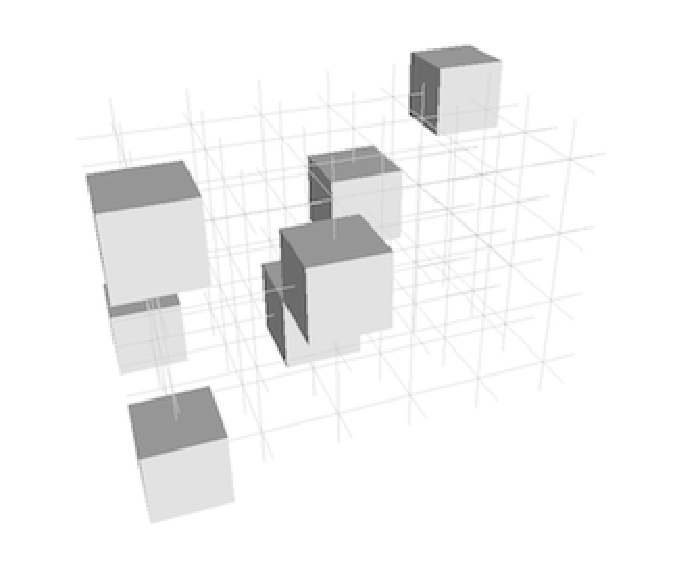
\includegraphics[width=0.3\textwidth]{Images/visuModeDefault.eps}&
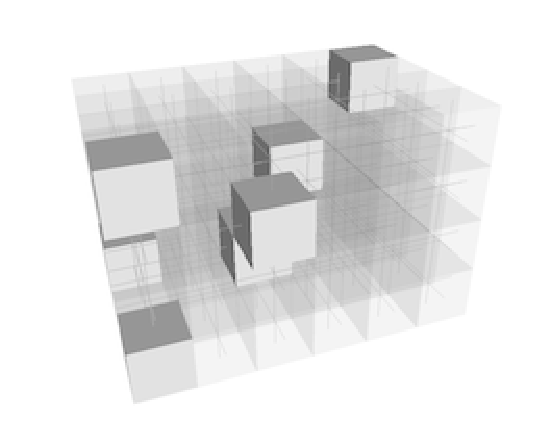
\includegraphics[width=0.3\textwidth]{Images/visuModePavingGridsDomain.eps}&

\includegraphics[width=0.3\textwidth]{Images/visuModeGridVoxel.eps}\\
mode  "" (Default) &  mode ``PavingGrids'' & mode ``Grid''
\end{tabular}
\end{center}

\end{frame}






\begin{frame}[t]

\frametitle{3. Modes de visualisation 3D }

\begin{block}{Visualisation personnalis�e}
\begin{semiverbatim}
viewer  \texttt{< \hspace{-0.2cm}<} CustomColors3D(Color(250, 0,0),Color(250, 0,0));
\end{semiverbatim}

\begin{center}
\includegraphics[width=0.6\textwidth]{Images/visuModeCustom-1.eps}
\end{center}
\end{block}
\end{frame}




\begin{frame}[t]
\frametitle{Exemples sur d'autres primitives }

\begin{center}
\begin{tabular}{c@{}c@{}c}
\includegraphics[height=0.22\textwidth]{Images/autrePrimitive3.eps}&
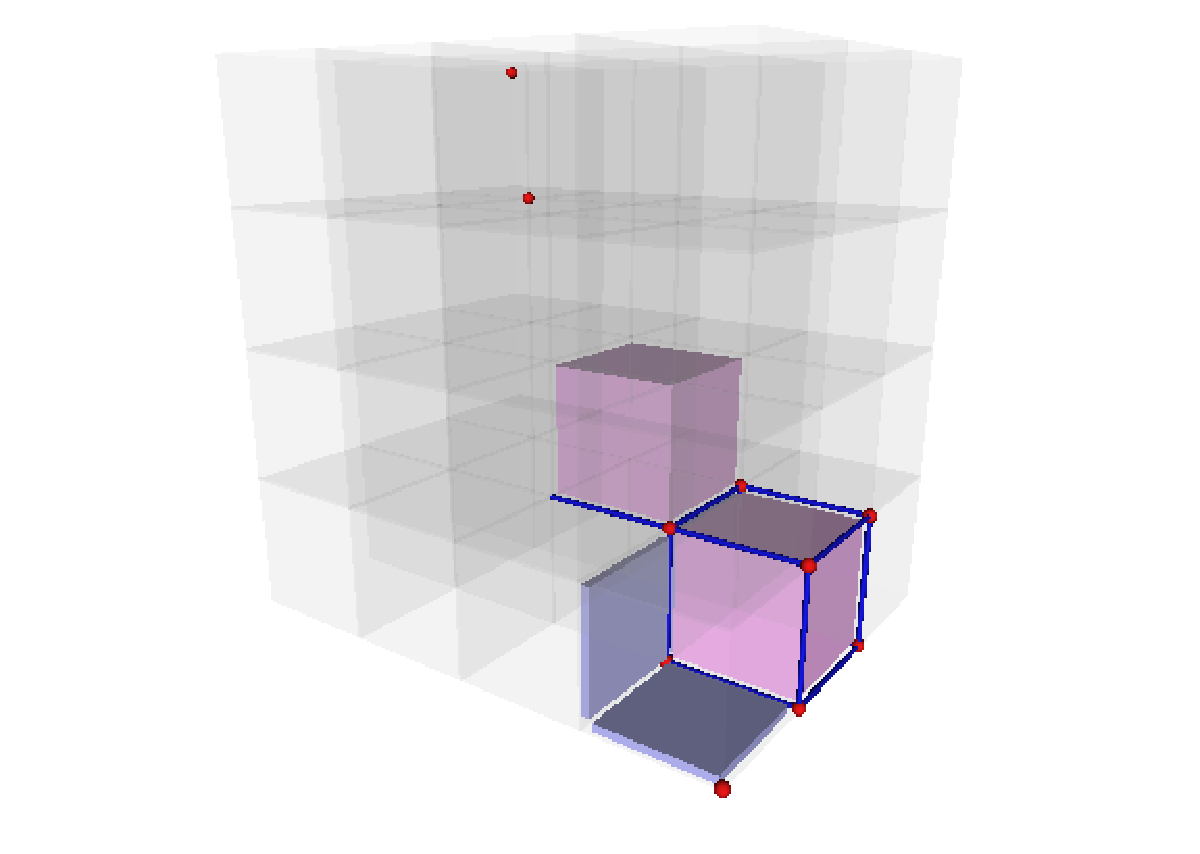
\includegraphics[height=0.22\textwidth]{Images/autrePrimitive2.eps}&
\includegraphics[height=0.22\textwidth]{Images/autrePrimitive.eps}\\
{\scriptsize{\class{Object} mode ``DrawAdjacencies''}} &{\scriptsize{\class{Khalimsky} Cells }}  & 
{\scriptsize{Signed \class{Khalimsky} Cells }} \\
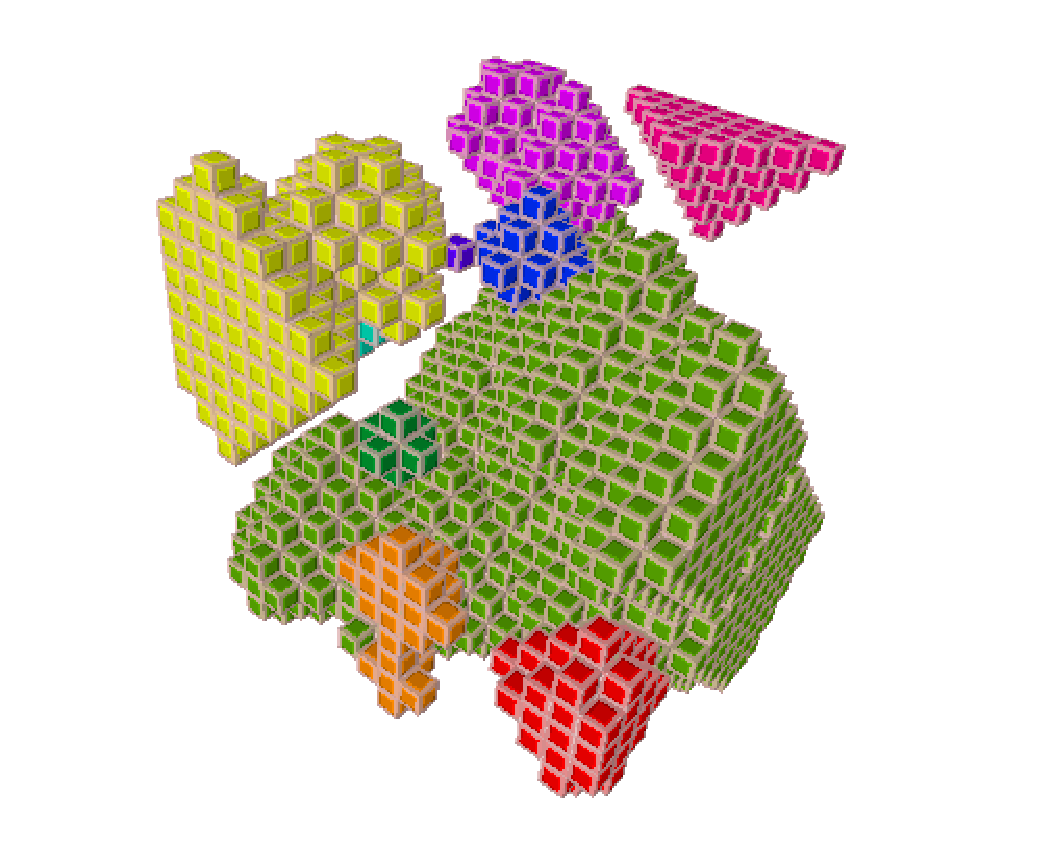
\includegraphics[height=0.22\textwidth]{Images/KSurfelsConnectedOrientExt.eps} &
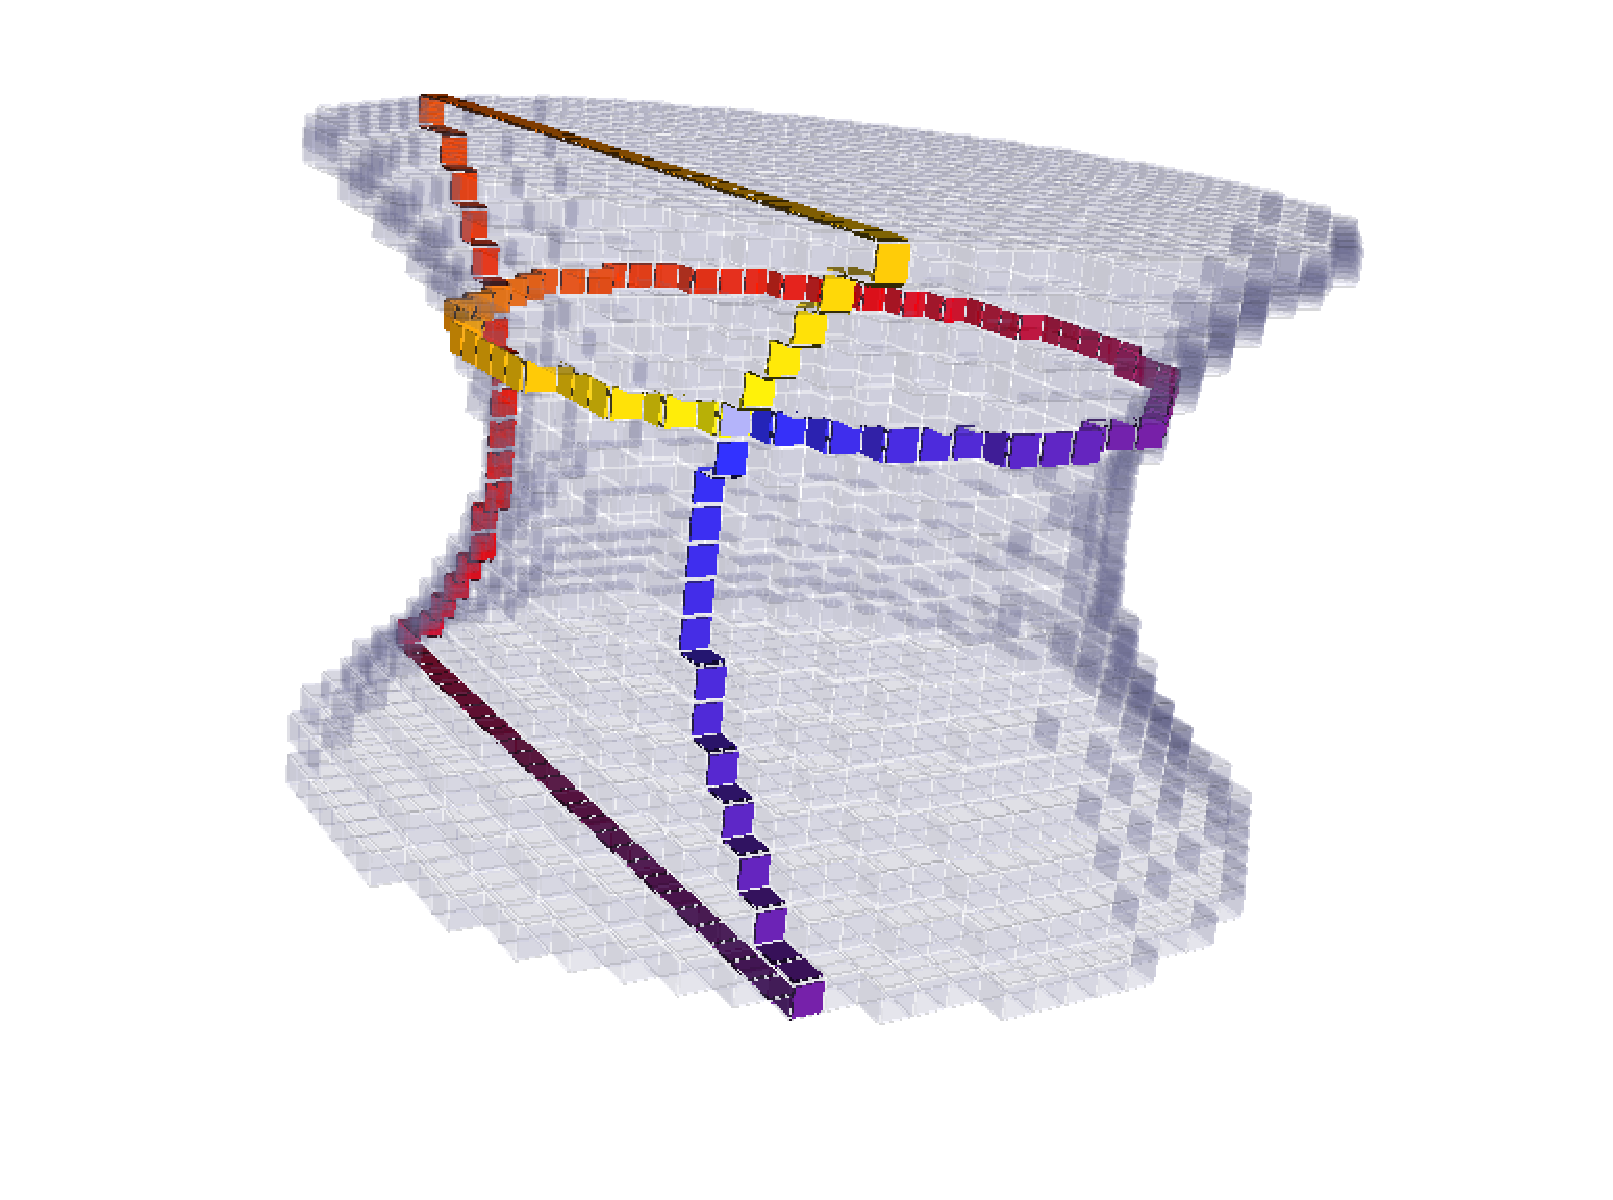
\includegraphics[height=0.22\textwidth]{Images/surfelTracking.eps}&
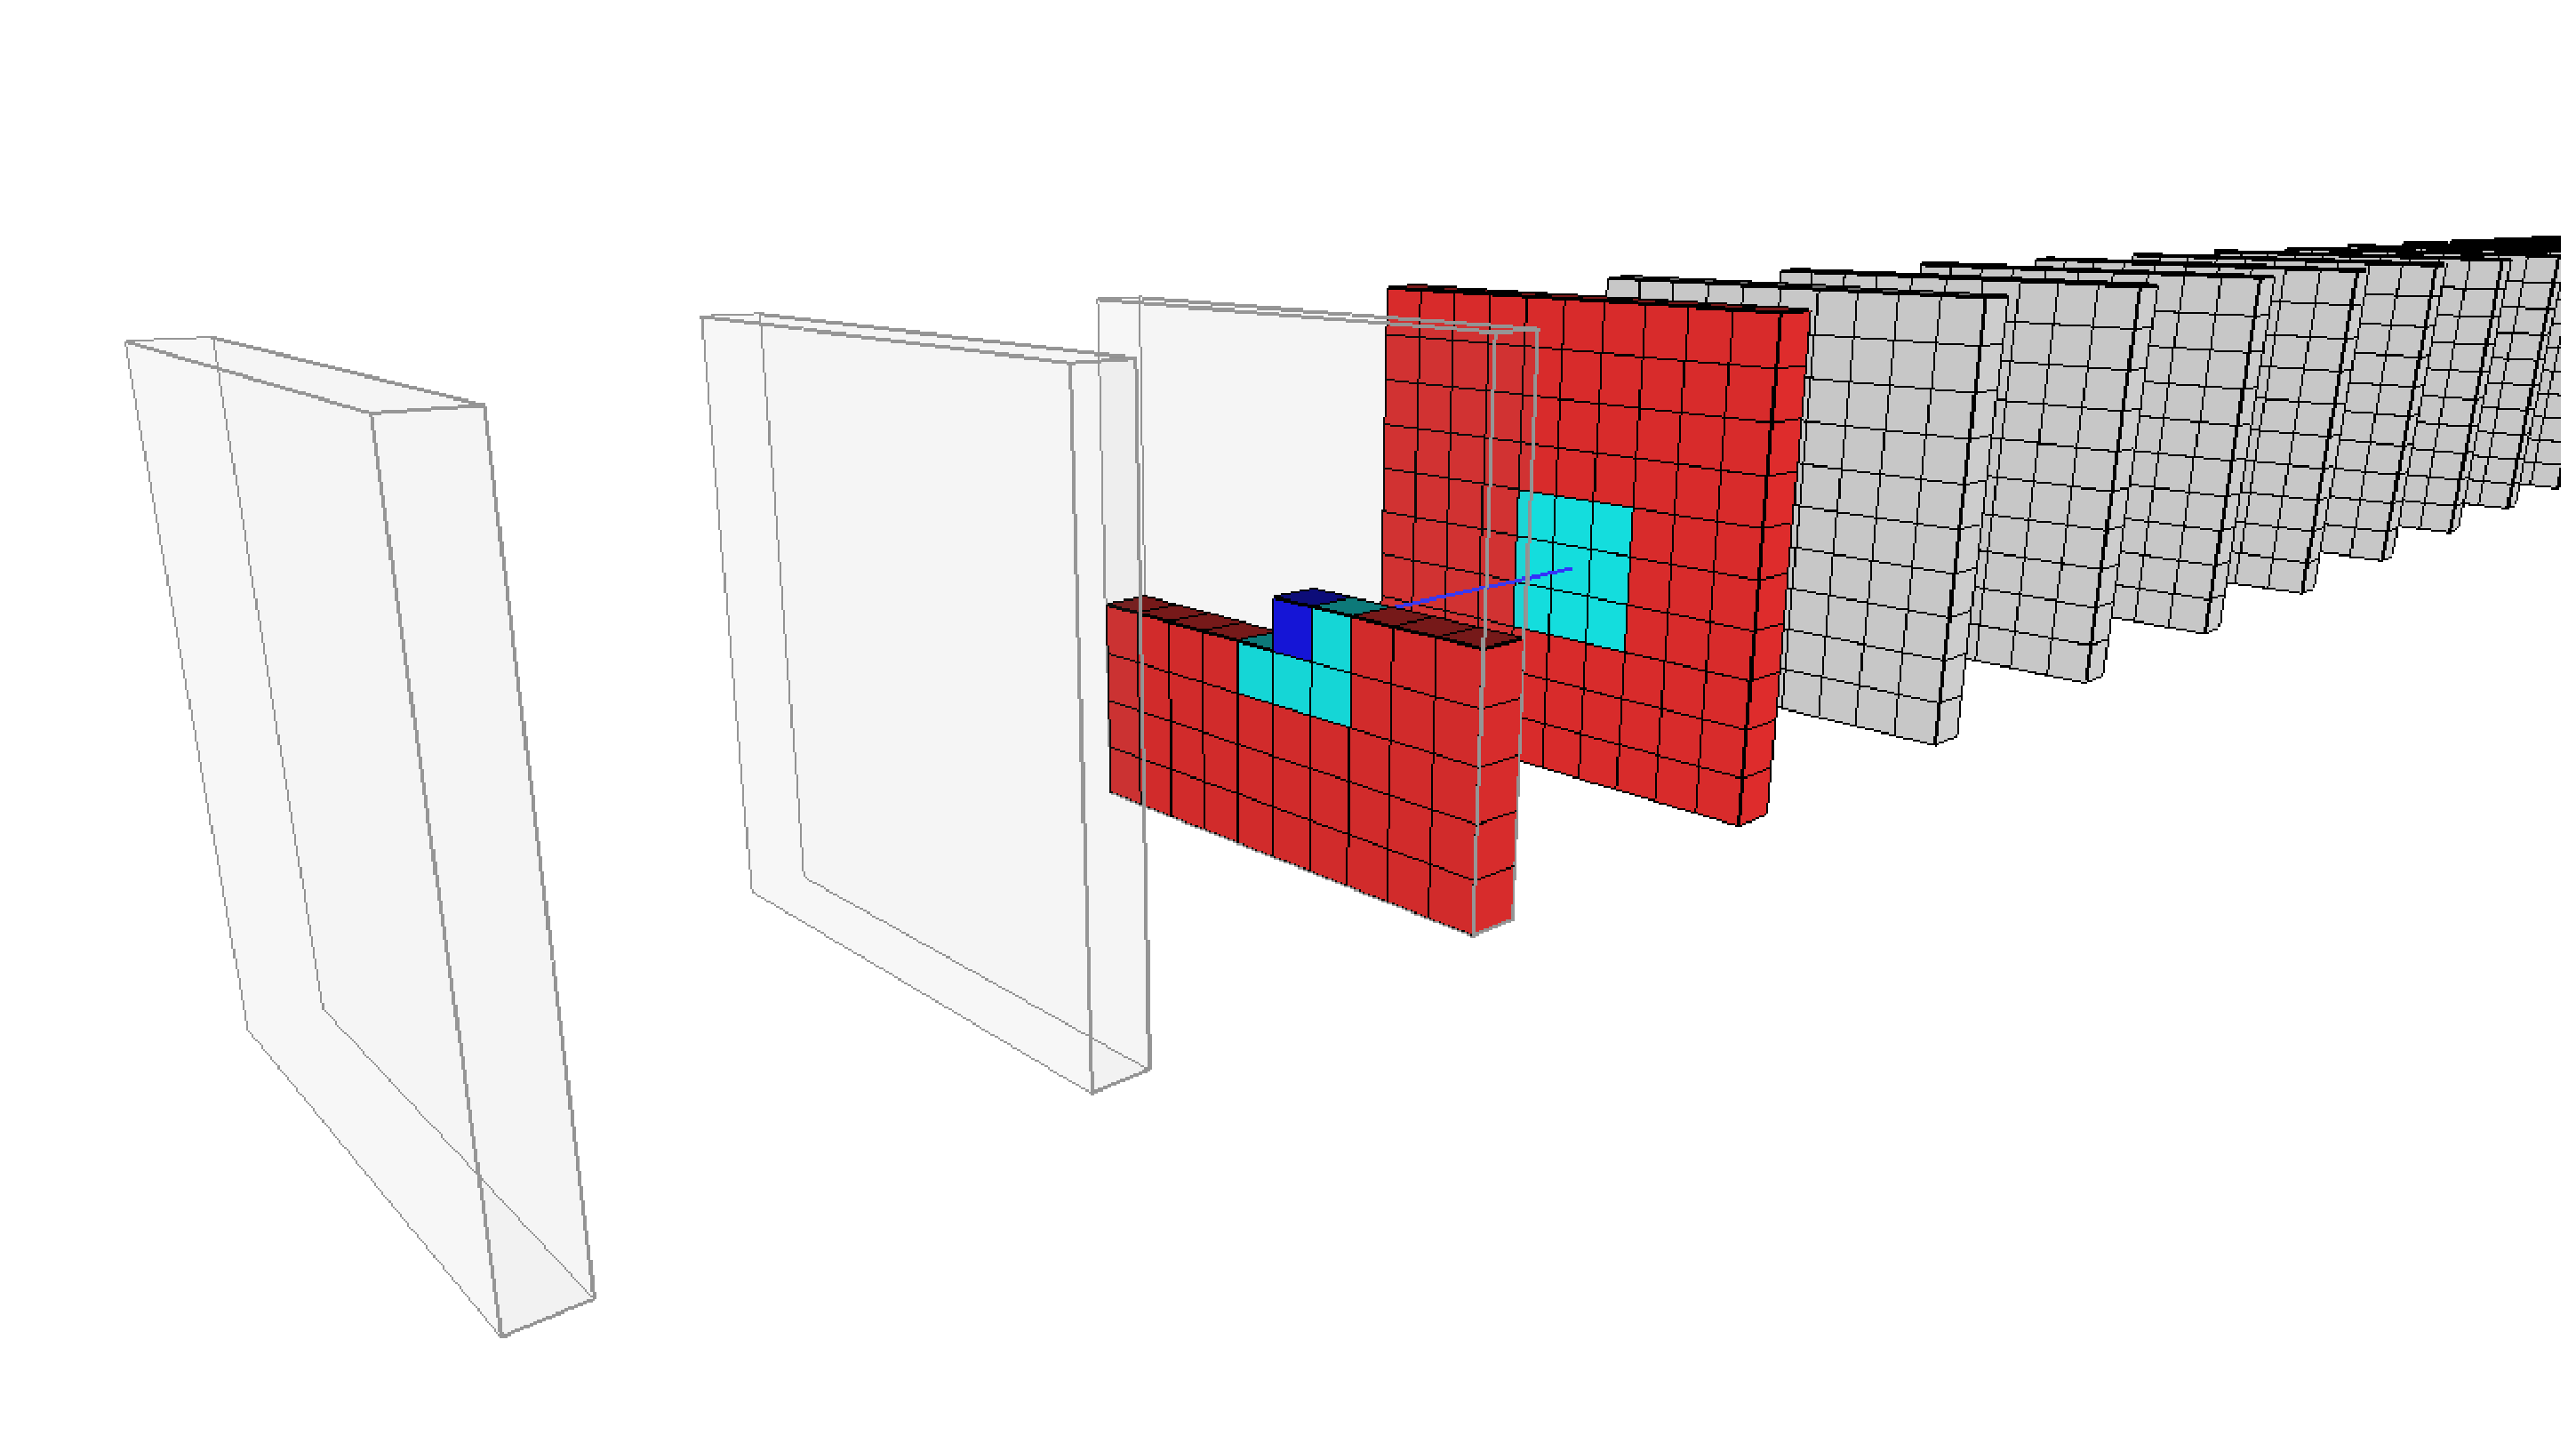
\includegraphics[height=0.2\textwidth]{Images/illustration3Dscan.eps} \\
{\scriptsize{Composantes connexes }}  & {\scriptsize{Suivi de surfels }} 

\end{tabular}
\end{center}


\end{frame}



\begin{frame}[t]
\frametitle{Autres fonctionnalit�s}

\begin{minipage}{0.65\textwidth}
\begin{block}{}
\begin{itemize}
\item Clipping planes: \\
\begin{semiverbatim}
 viewer  \texttt{< \hspace{-0.2cm}<} ClippingPlane(1,0,0,-4.9);
 viewer  \texttt{< \hspace{-0.2cm}<} ClippingPlane(0,1,0.3,-10); 
\end{semiverbatim}
\item<3-> Importation de donn�es simplifi�e (visu volumique en moins de 50 lignes)..
\item<4-> Gestion de la transparence.
\end{itemize}

\end{block}
\end{minipage}
\only<1>{\rput(2.2,0){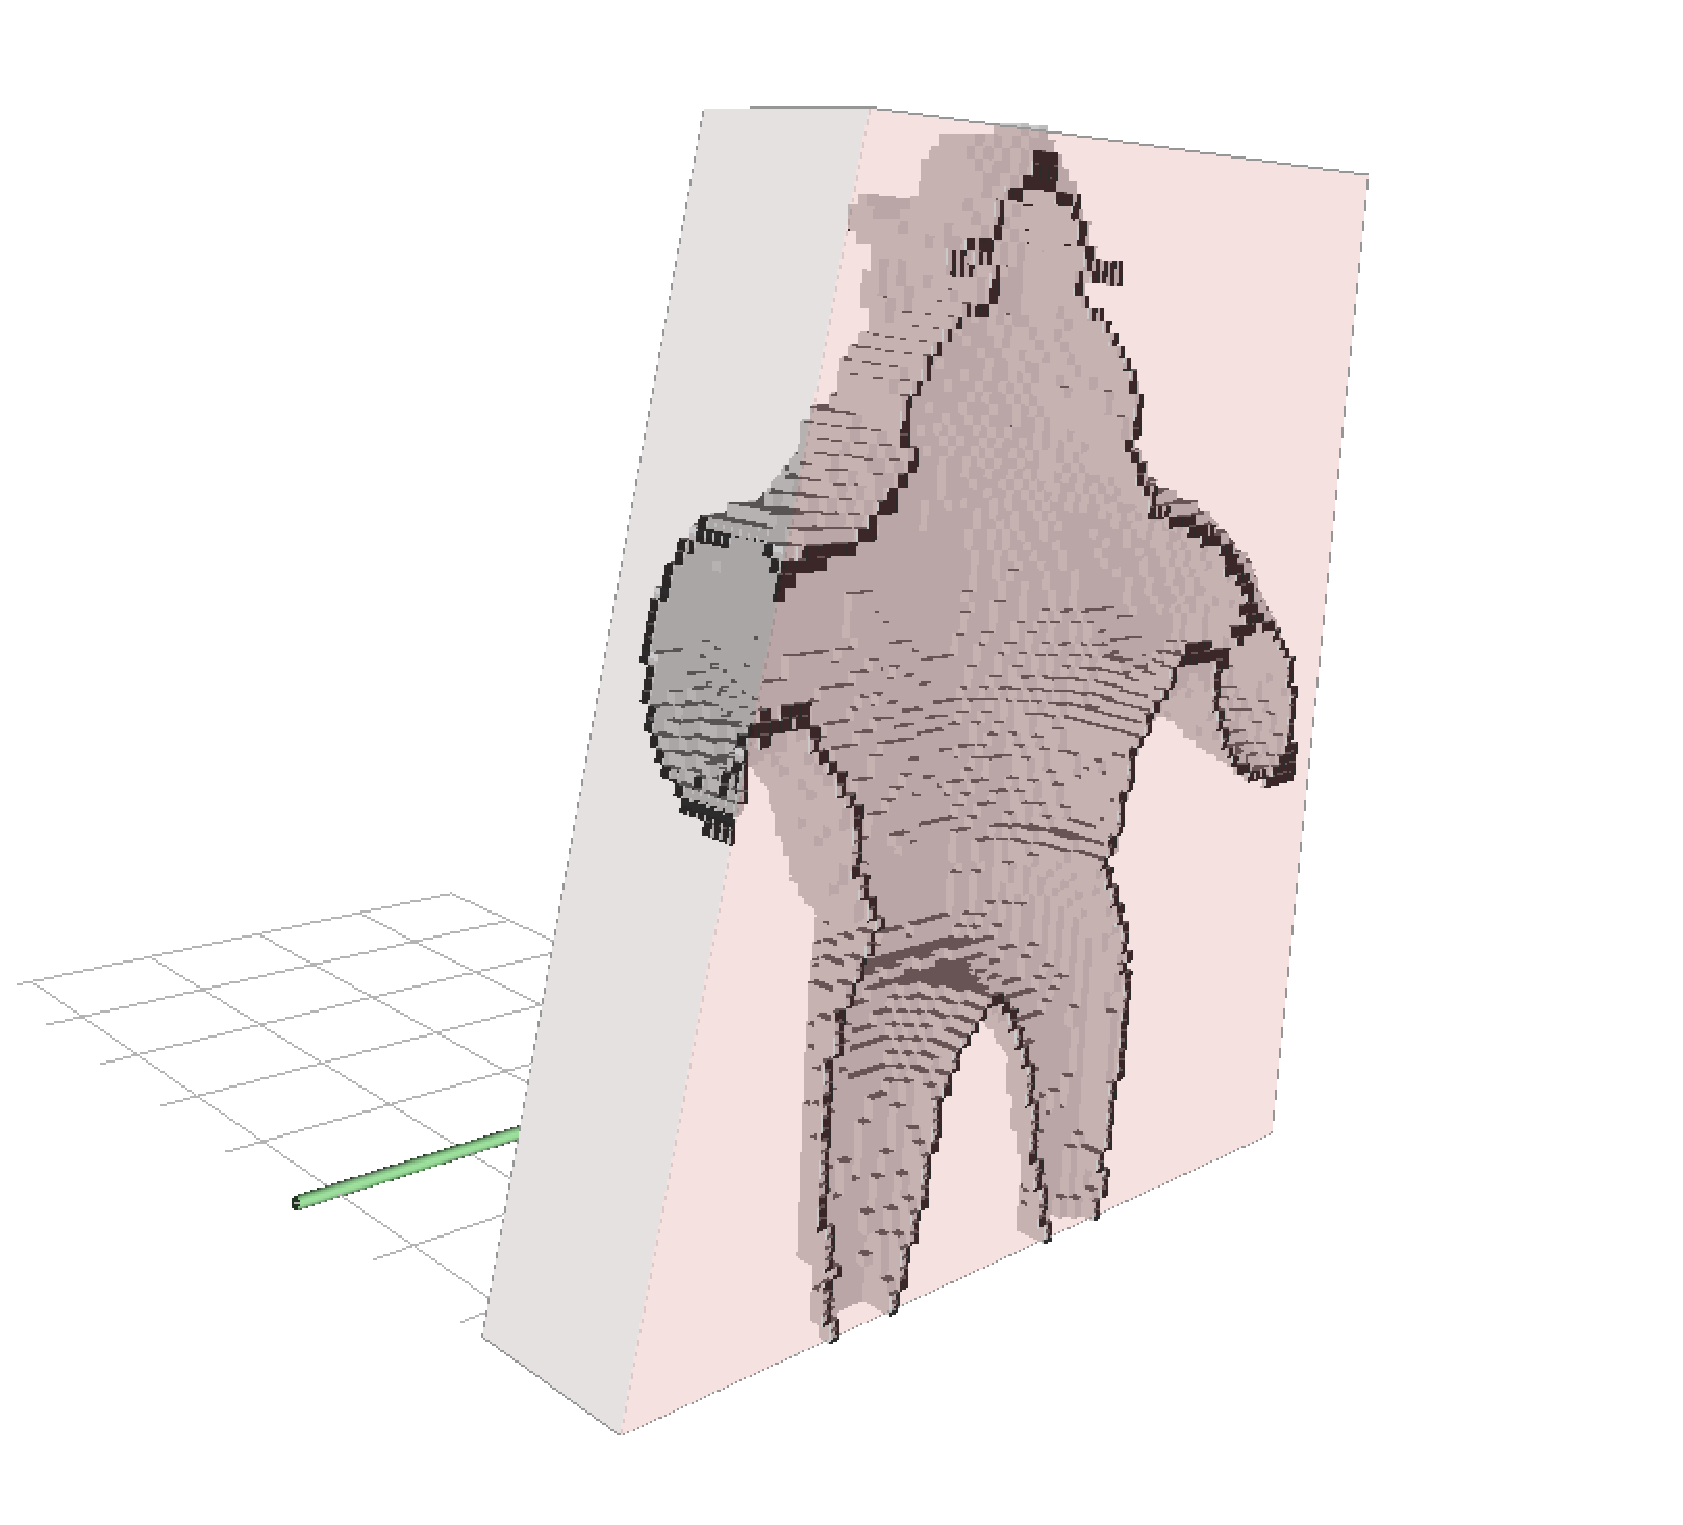
\includegraphics[width=0.3\textwidth]{Images/clipping1.eps}}}%
\only<2->{\rput(2.2,0){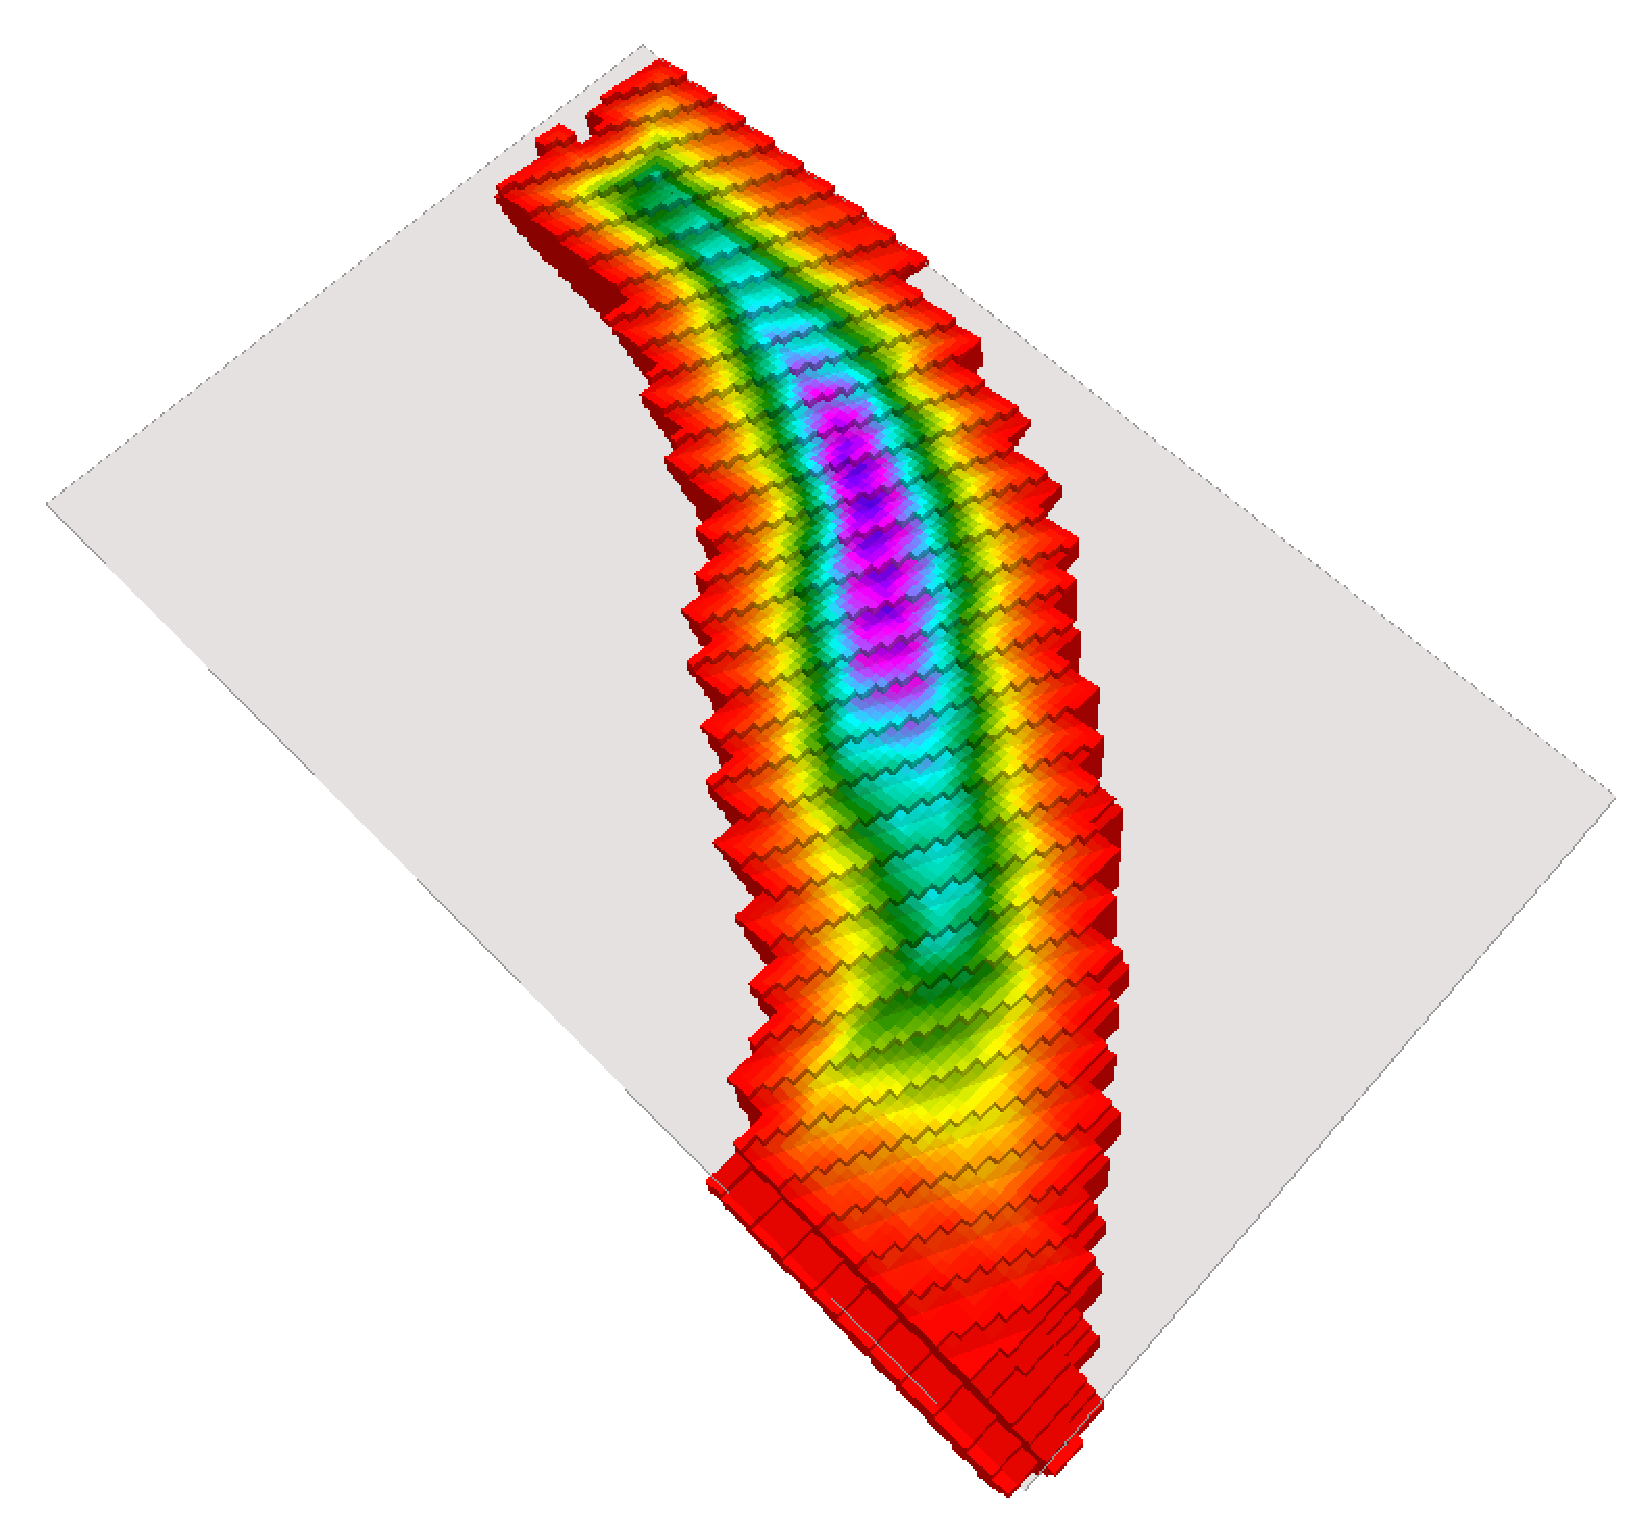
\includegraphics[width=0.3\textwidth]{Images/distanceMap.eps}}}%
\only<3>{\rput(-1.5,-3.6){\includegraphics[width=0.4\textwidth]{Images/visuVol3.eps}}}%
\only<4>{\rput(-1.5,-3.6){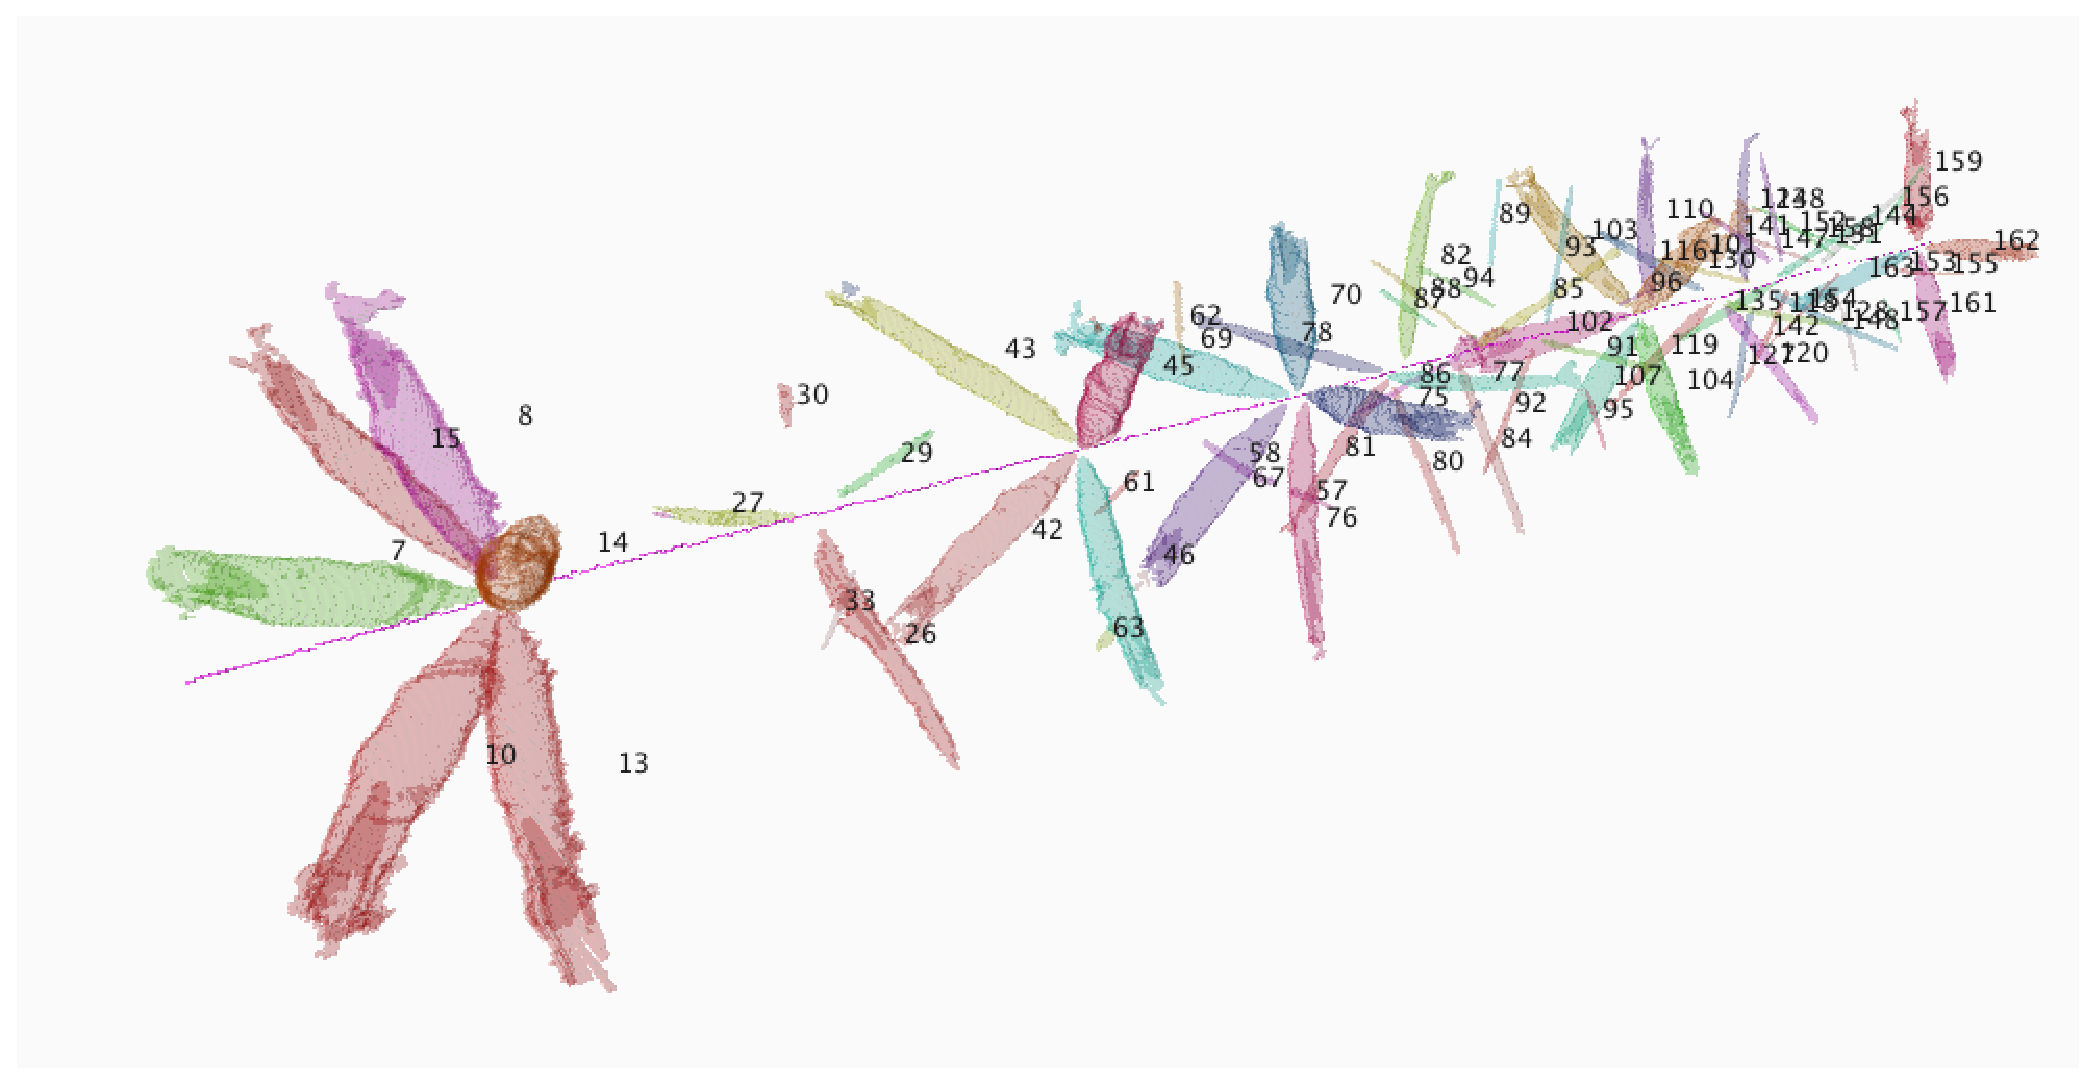
\includegraphics[width=0.6\textwidth]{Images/branche.eps}}}%

\end{frame}



\begin{frame}[c]
\frametitle{Exemple du code de l'outil de visualisation:}

\begin{center}
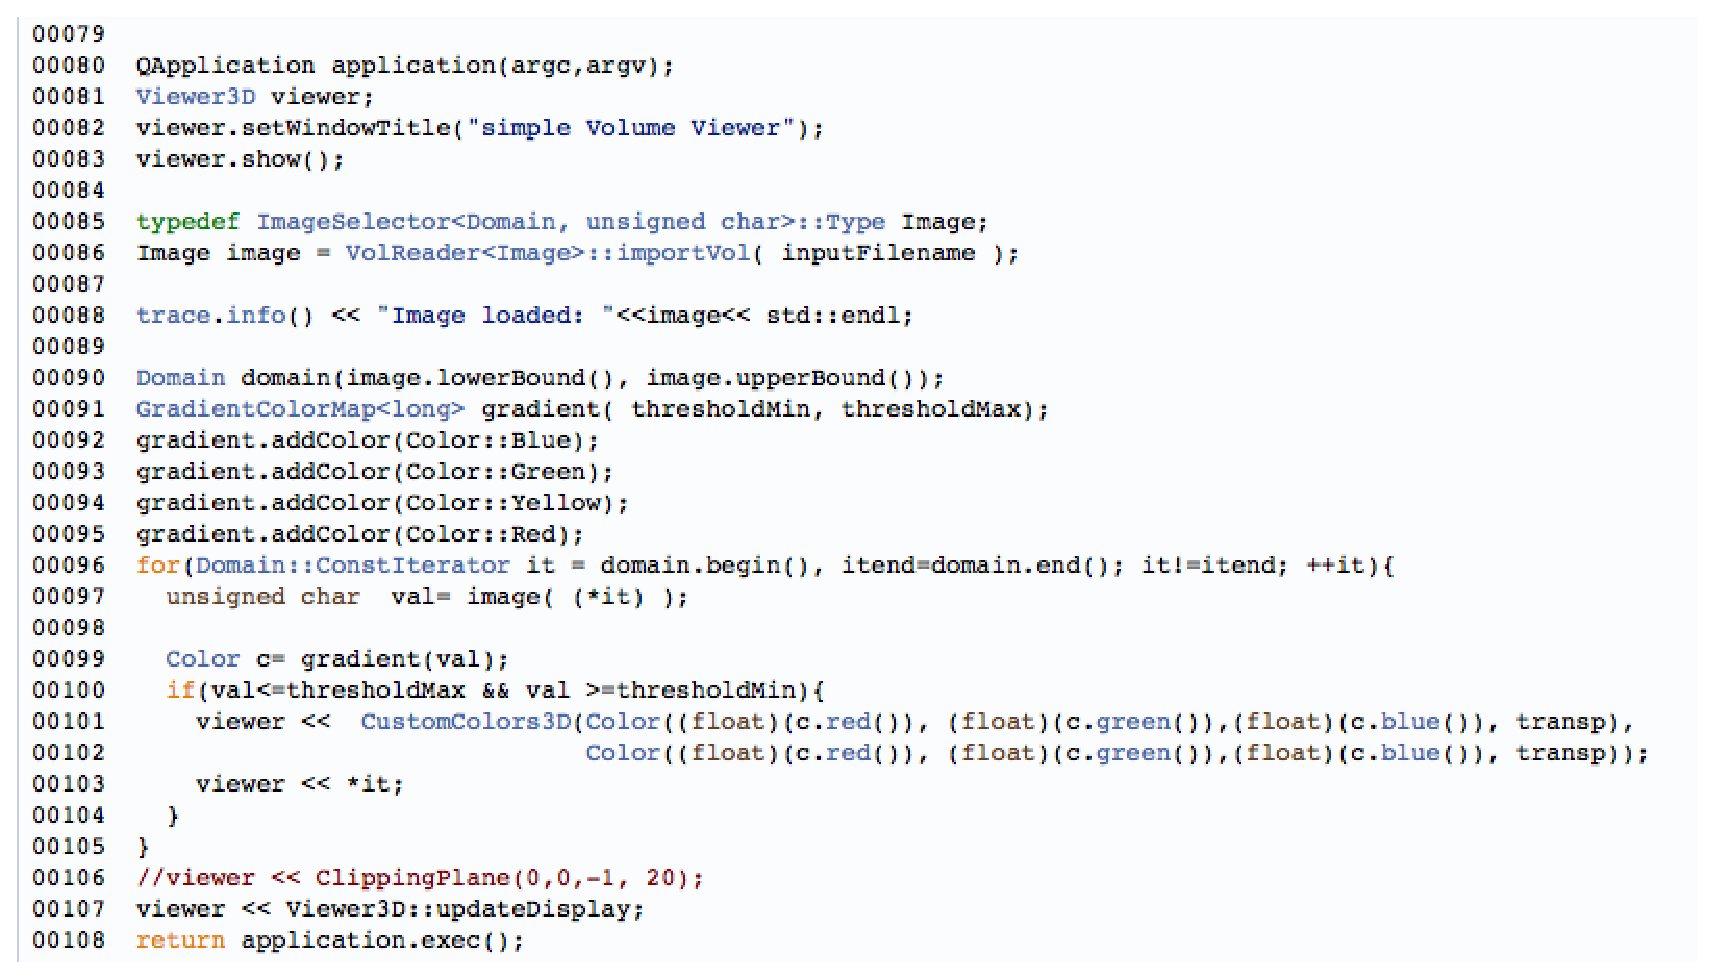
\includegraphics[width=0.9\textwidth]{Images/codeVisu3D.eps}
\end{center}


\end{frame}



\section{4. Travail restant}



\begin{frame}[t]
\frametitle{4. Travail restant}

\begin{itemize}
\item Modifier le principe \texttt{``SelfDraw()''}. 
\item Terminer l'harmonisation entre \class{Board2DTo3D} et \class{Viewer3D}.
\item Rajouter des mod�les de r�flectance dans \class{Board2DTo3D}.
\item Corriger partiellement l'export vectoriel bas� \class{Viewer3D} (de
  LibQGLViewer: biblioth�que \texttt{VRender} de Cyril Sole).
\end{itemize}
\end{frame}





\begin{frame}
  \frametitle{4. Travail restant: visu en PDF 3D ? :(issue \#35) }

\begin{block}{Export en format U3D :}
  \begin{center}
\only<1> {
    \includemovie[
    poster,
    label=example.u3d,
    text=(example.u3d : click to display),
    3Daac=60.000000, 3Droll=0.000000, 3Dc2c=-3295.047852 248.228210 -1028.702759, 
    3Droo=3460.807129, 3Dcoo=-3.445007 -0.000031 1.349976,
    3Dlights=CAD,
    ]{.5\linewidth}{.5\linewidth}{example.u3d} }%%
\only<2>{
\begin{semiverbatim}
    poster,label=example.u3d, 

    text=(example.u3d : click to display),

    3Daac=60.000000, 3Droll=0.000000, 3Dc2c=-3295.047852 
    
    248.228210 -1028.702759, 3Droo=3460.807129, 
    
    3Dcoo=-3.445007 -0.000031 1.349976,

    3Dlights=CAD,

    ]{3cm}{3cm}{example.u3d}
\end{semiverbatim}}

  \end{center}

\end{block}

\end{frame}








\end{document}



